\clearpage
\section{Grundlagen}
\label{sec:2}
In diesem Kapitel wird auf die Grundlagen der in diesem Beleg verwendeten Technologien eingegangen.

\subsection{Grundlagen Smartcard}
\label{subsec:2.1}
Die in diesem Beleg verwendete Smartcard basiert auf der Java Card Technologie. Die Java Card Technologie bietet eine 
Teilmenge der Java Programmiersprache, sowie eine hinsichtlich der Anforderungen an Smartcards optimierte Laufzeitumgebung.

Die Verwendung von Java-basierten Smartcards bietet einige Vorteile, von denen nachfolgend eine Auswahl beispielhaft genannt sei: \cite{jcopdoc}

\begin{description}
\item[plattformunabhängig:] Java Card Applets, die der Java Card API entsprechen, lassen sich plattformunabhängig und herstellerübergreifend nutzen.
\item[Multiapplikationsfähig:] es können mehrere Applikationen gleichzeitig auf einer Smartcard ausgeführt werden
\item[hohe Flexibilität:] die Verwendung der objektorientierten Programmiersprache Java erlaubt die Erstellung komplexer Anwendungen für die Smartcard.  
\item[Post-Aktualisierbarkeit:] die Möglichkeit, nachträglich Code auf der Smartcard zu modifizieren und auszutauschen erhöht die Flexibilität weiter
\item[Standardkonformität:] die Java Smartcards entsprechen dem ISO7816 Standard \cite{iso7816}
\end{description}

Eine Java Smartcard besteht im Wesentlichen aus den Bestandteilen Kommunikationsschnittstelle, Speicher und einem Prozessor zur Durchführung von Berechnungen.
Bei Verwendung der Smartcard wird diese in ein Lesegerät eingelegt. Das Lesegerät wird in einschlägiger Literatur auch als Card Acceptance Device, abgekürzt CAD, bezeichnet.
Der Speicher auf Java Smartcards besteht aus zwei Typen, RAM und EEPROM. Der RAM-Speicher ist flüchtig und kann beliebig oft beschrieben werden. Der EEPROM-Speicher ist nichtflüchtig und kann nur endlich oft beschrieben werden, je nach Hersteller und Modell bis zu 100.000 mal pro Speicherzelle.  

\subsection{JCOP}
\label{subsec:2.2}
JCOP ist eine kontextorientierte Programmiererweiterung für die Programmiersprache Java und kombiniert COP-Vorteile mit neuen Konstrukten wie ereignisorientierten und deklarativen Layerkompositionen.

\subsection{APDU}
\label{subsec:2.3}

Die Kommunikation zwischen dem Kartenlesegerät und der Smartcard erfolgt reaktiv und paketweise. Reaktiv bedeutet, dass die Smartcard keine Kommunikation initiiert sondern nur auf Anfragen vom Lesegerät reagiert. Der bei der Kommunikation zwischen Smartcard und Lesegerät verwendete Kommunikationsmechanismus wird als Application Protocol Data Units, abgekürzt APDU, bezeichnet. Spezifiziert ist dies ebenfalls in ISO7816 Teil 4.\cite{iso7816}
\\

\begin{figure}[htb]
\begin{center}
 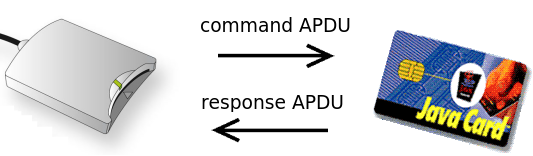
\includegraphics[width=1\hsize]{./images/apdu.png}
\end{center}
\caption[APDU-Kommunikation schematisch dargestellt, Quelle: Autoren]{\label{apdu}APDU-Kommunikation schematisch dargestellt, Quelle: Autoren}
\end{figure}

Die Kommunikation wird über ein so genanntes command APDU Paket initiiert, welches aus den folgenden Feldern besteht:


\begin{description}
\item[CLA:] class,gibt die Klasse an, spezifiziert ob es sich um ein ISO7816-4 konformes Kommando handelt
\item[INS:] gibt die Instruktion an
\item[P1:] zusätzlicher Parameter
\item[P2:] zusätzlicher Parameter
\end{description} 

Weiterhin können je nach Kommandotyp noch die folgenden, optionalen Felder an das command APDU Paket angehängt werden:

\begin{description}
\item[Lc:] Length, gibt die Länge der Kommandodaten
\item[Data:] gibt die Kommandodaten an
\item[Le:] gibt die Länge der erwarteten Antwort an
\end{description}

Als Antwort erhält das Lesegerät von der Smartcard ein so genanntes response APDU Paket. Dieses Antwortpaket kann ein Datenfeld enthalten, dies ist jedoch nicht obligatorisch. Das response APU Paket ist wie folgt aufgebaut.

\begin{description}
\item[Data:] optionales Datenfeld
\item[Sw1:] Statusword, erstes Byte
\item[Sw2:] Statusword, zweites Byte
\end{description}




